\documentclass[tikz,border=10pt]{standalone}
\usetikzlibrary{calc}
\begin{document}
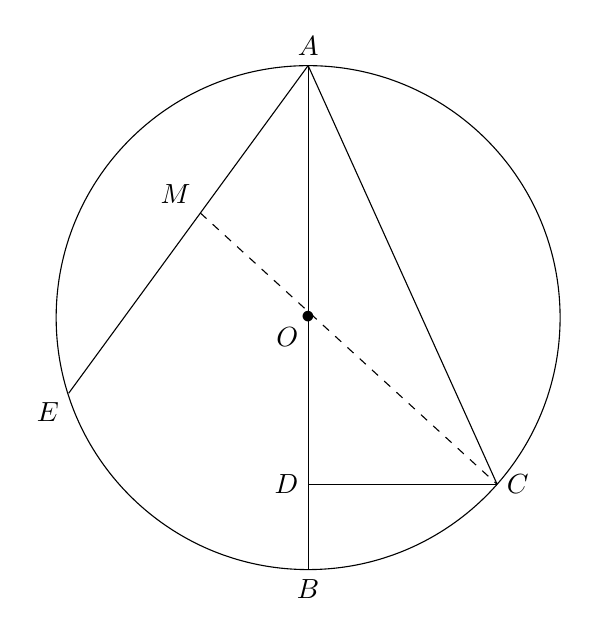
\begin{tikzpicture}[scale=1.6]
  \coordinate (O) at (0,0);
  \coordinate (A) at (0,2);
  \coordinate (B) at (0,-2);
  \coordinate (C) at (1.5,-1.3229);
  \coordinate (E) at (-1.9,-0.6);
  \coordinate (D) at (0,-1.3229);
  \coordinate (M) at ($(A)!0.45!(E)$);

  \draw (O) circle (2);
  \draw (A) -- (B);
  \draw (A) -- (E);
  \draw (A) -- (C);
  \draw (D) -- (C);
  \draw[dashed] (M) -- (C);

  \node at (O) {$\bullet$};

  \node[above] at (A) {$A$};
  \node[below] at (B) {$B$};
  \node[right] at (C) {$C$};
  \node[below left] at (E) {$E$};
  \node[left] at (D) {$D$};
  \node[below left] at (O) {$O$};
  \node[above left] at (M) {$M$};
\end{tikzpicture}
\end{document}
